
An intrinsic problem with SOMs in two dimensions is the so called edge
effect. This is illustrated in  in Figure \ref{f:edge}, which displays a SOM
trained on socioeconomic census data consisting of 32 variables for US states.
The darker a neuron in the figure, the larger is the distance between the
 neuron and mean of the input vectors. The distance between each of the
 original observations (states) and the mean is represented by a graduated
 circle. Taking these two together it is clear that the outlier observations
 are pushed towards the edges of the map, while the observations that are
 closest to the multidimensional center of the data are assigned to central
 neurons on the map.

At the edge of the map, neurons have fewer neighbors which results in any
observations being assigned to them having fewer competitive signals. At the
same time, the edge of the neural lattice represents a true visual boundary
which affects its ability to represent data similarities as spatial
relationships.

\begin{figure}
  \begin{center}
\caption{Edge effects in SOM}\label{f:edge}
  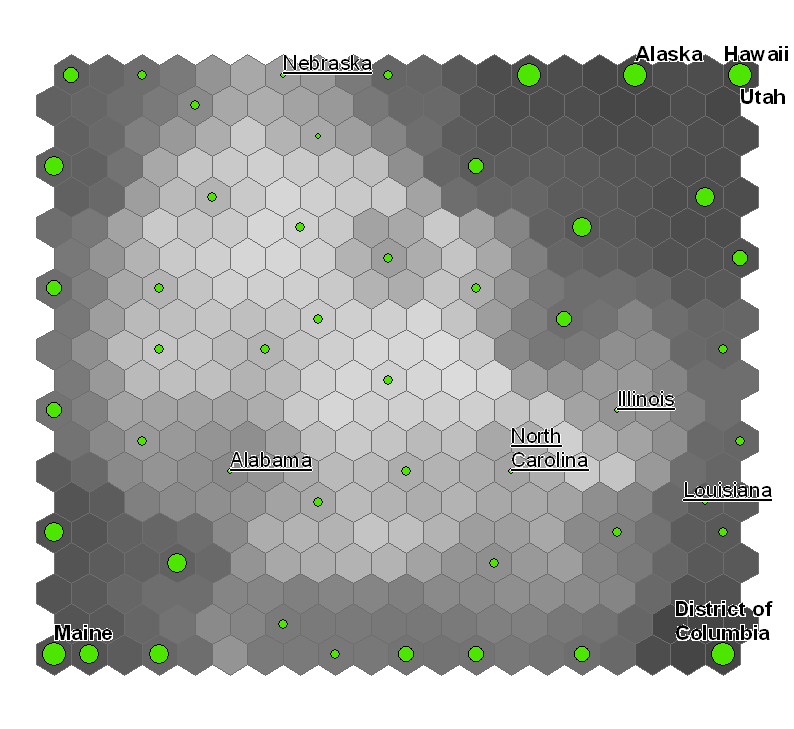
\includegraphics[width=0.70\linewidth]{states.png}
\end{center}
\end{figure}

One way to eliminate the edge effect is to wrap the lattice around a
three-dimensional object such as a sphere or torus, thereby removing the edge
entirely. The toroidal SOM was introduced by Li et al. \cite{li1993}, however the torus
is not effective for visualization, as maps generated from a torus are not
very intuitive \cite{ito2000,wu2006}.  Ritter \cite{ritter99} describes the torus as
being topologically flat and suggests that a curved topology, such as that of
a sphere, may better reflect directional data.  A sphere also results in a
more intuitive map, since we are accustomed to looking at geographic maps
based on a sphere.  

\label{bg:sphere}
Ritter \cite{ritter99} first introduced the spherical SOM, and several enhancements have
since been suggested \cite{boudjemai2003,sangole03,Nishio:2006fk,wu2006}.  A
good comparison of these enhancements can be found in Wu and Takatsuka
 \cite{wu2006}.  All of
these methods derive their spherical structure through the tessellation of a
polyhedron as originally proposed by Ritter \cite{ritter99}.  Wu and Takatsuka \cite{wu2006} point
out the importance of a uniform distribution on the sphere, and that it is
preferable for all neurons to have an equal number of neighbors and to be
equally spaced.  They find generally that the tessellation method best satisfies
these conditions, and specifically that the icosahedron is the best starting
point \cite{wu2005}. Tessellation of the icosahedron results in a network of
neurons, each having exactly six neighbors, save the original twelve
which each have five neighbors.  This is very close to the ideal structure in
which every neuron would have exactly six neighbors.  Wu and Takatsuka \cite{wu2006} prefer
this structure, because it has very low variances in both neuron spacing
and neighborhood size. 

Based solely on measures of neuron spacing, Wu and Takatsuka \cite{wu2005} dismissed the usefulness of a method
proposed by Rakhmanov et al. \cite{Rakhmanov94} for distributing points on a sphere.
Similarly Nishio et al.
\cite{Nishio:2006fk} use these variance measures to support their helix
algorithm for distributing points on a sphere.  However,
these metrics can be misleading and comparison across topologies may not be
consistent.  The traditional rectangular and hexagonal topologies have no
variance in neuron spacing, and the generally preferred hexagonal structure
displays greater variance in neighborhood size than the rectangular structure.
The torus, by comparison, would have variance in neuron spacing, yet no
variance in neighborhood size.  The distance between two neurons is only
considered during the formation of the neural network.  At this stage the
spacing is significant as it plays a part in constructing the network's
topology by determining neuron adjacency.  However, using this measure to
evaluate potential topologies for use in SOM may be misleading.

As spherical (and other alternative) topologies become
increasingly more common it is necessary to investigate how the choice of
topology effects the SOM.  In this paper the effect of irregularity within
topologies is studied as an attempt to investigate not only the edge effect,
but also to help facilitate the comparison of topologies.  It is important to
note that spherical topologies may not be appropriate for all applications.
Removing the edge may reduce the SOM's ability to converge.  As outliers are
forced to interact they introduce more competition among the neurons.  We
would also expect outliers to occupy more space in the final map as their
dissimilarity in attribute space should translate to more distant spatial
relationships in the trained SOM.  More research will be needed to help researches
determine the most appropriate topology for their data and research objectives.

In this paper we explore the general utility of certain irregular spherical
topologies beyond offering greater control over network size. We develop and
test new diagnostics to measure and visualize topology-induced errors in SOM.
More specifically we 

\begin{enumerate}
\item Compare the internal heterogeneity of observations captured by a given neuron to that neuron's first-order neighborhood size.
\item For different topologies, compare the internal heterogeneity of each neuron against a composite measure of topological regularity.
\item Develop a SOM-based visualization of the internal heterogeneity.
%\item Develop a reverse quantization error visualization by mapping neurons back onto the input data.
\end{enumerate}

These diagnostics help facilitate the evaluation of both traditional and
spherical SOMs. To satisfy the objective of this research, we apply these
diagnostics to a series of comparable SOMs. Each SOM is trained using the
same synthetic data and training parameters, but utilize different network
topologies. By formally testing for difference of means and variance in the
results of the diagnostics, the following questions are addressed:

\begin{enumerate}
\item Does the internal heterogeneity of a neuron decrease as its first-order neighborhood size, or degree, increases?
\item Is the average internal heterogeneity of a SOM higher when a more irregular topology is used?
\item Which insights, if any, can be gained from a SOM-based visualization of internal heterogeneity?
\end{enumerate}


